
\includegraphics[height=1.25cm]{images/pictograms/replication}
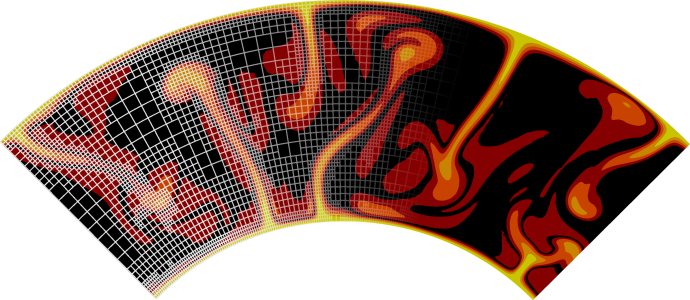
\includegraphics[height=1.25cm]{images/pictograms/aspect_logo}

\includegraphics[height=1.25cm]{images/pictograms/benchmark}

\includegraphics[height=1.25cm]{images/pictograms/under_construction}

\includegraphics[height=1.25cm]{images/pictograms/FEM}
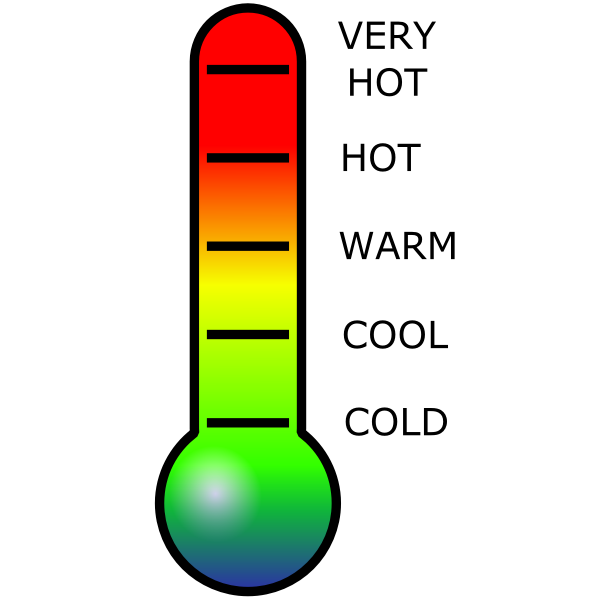
\includegraphics[height=1.25cm]{images/pictograms/temperature}

%%%%%%%%%%%%%%%%%%%%%%%%%%%%%%%%%%%%%%%%%%%%%%%%%%%%%%%%%%%%%%%%%%%%%%%%%%%%%%%%%%%%%%%%%%%%%%%%%%%

\begin{flushright} {\tiny {\color{gray} python\_codes/fieldstone\_149/text.tex}} \end{flushright}

\lstinputlisting[language=bash,basicstyle=\small]{python_codes/fieldstone_149/keywords.key}

\par\noindent\rule{\textwidth}{0.4pt}

\begin{center}
\inpython
{\small Code: \url{https://github.com/cedrict/fieldstone/tree/master/python_codes/fieldstone_149}}
\end{center}

\par\noindent\rule{\textwidth}{0.4pt}

{\sl This stone was developed in with input from Daniel Douglas}. 

\par\noindent\rule{\textwidth}{0.4pt}

%%%%%%%%%%%%%%%%%%%%%%%%%%%%%%%%%%%%%%%%%%%%%%%%%%%%%%%%%%%%%%%%%%%%%%%%%%%%%%%%%%%%%%%%%%%%%%%%%%%

In the {\pythonfile tools.py} there are two functions:
\begin{itemize}
\item \verb'merge_two_blocks': it takes as arguments two meshes and returns a single mesh in which 
the overlapping nodes of both have been merged and the global numbering and connectivity array computed.
\item \verb'export_to_vtu': it takes a mesh and exports it to vtu format.
\end{itemize}

%-------------------------------------------------
\section*{Joining two simple and identical meshes}

We start with two square meshes of resolution $20 \times 20$. This is implemented 
in {\pythonfile stone\_demo.py}.

\begin{center}
a)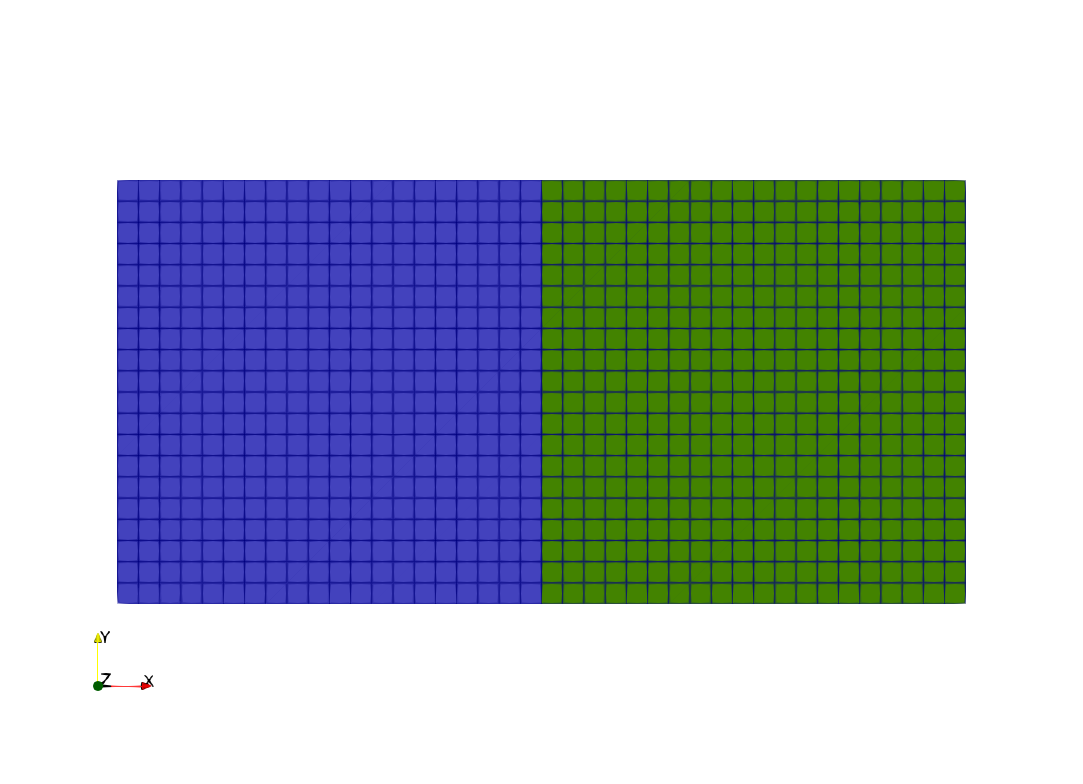
\includegraphics[width=8cm]{python_codes/fieldstone_149/results/one}
b)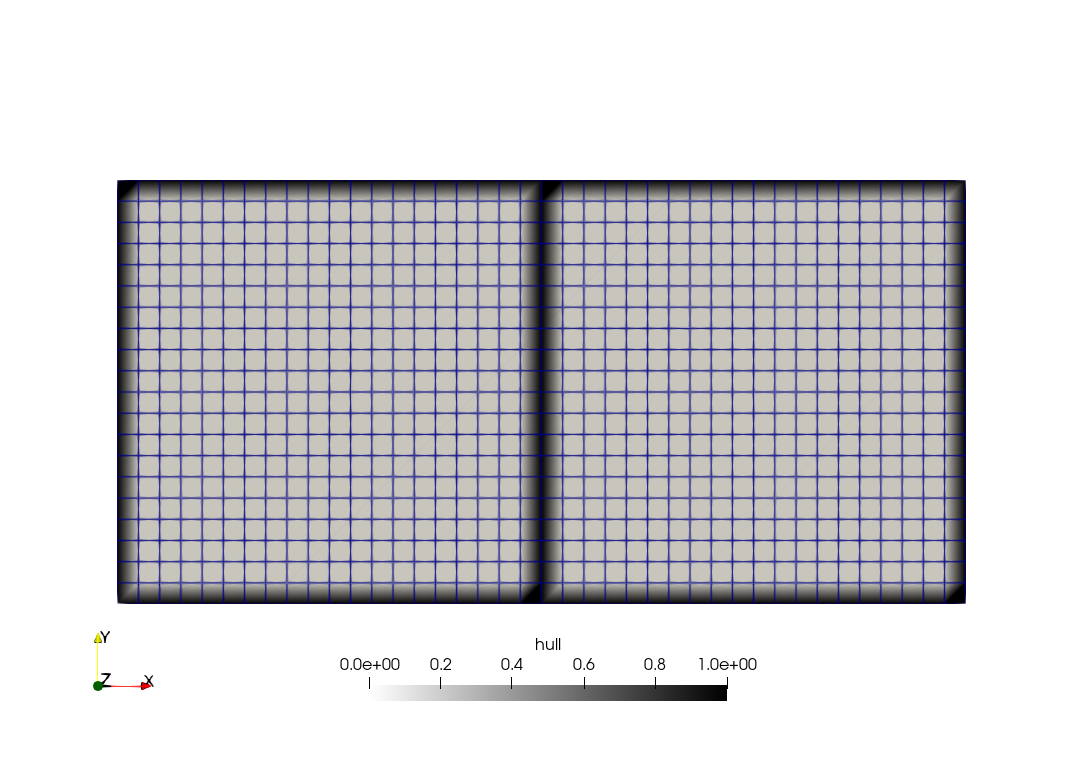
\includegraphics[width=8cm]{python_codes/fieldstone_149/results/two}\\
{\captionfont a) two individual meshes. b) final assembled mesh showing the hull flag. Note that the current algorithm does not unflag nodes that are no more on the boundary, it simply merges the two hull fields.}
\end{center}


%-------------------------------------
\section*{Joining multiple meshes}

This proto-mesh contains 8 elements and 14 points.

\begin{verbatim}
12---------------13
| \               |
|  10------------11 icon[0:m,0]=[0,1,6,5]
|   | \           | icon[0:m,1]=[1,2,7,6]
|   |  \          | icon[0:m,2]=[2,3,8,7]
|   |   \         | icon[0:m,3]=[3,4,9,8]
|   |    \        | icon[0:m,4]=[5,6,10,12]
5---6     8-------9 icon[0:m,5]=[6,7,8,10]    
|   | \-  / \     | icon[0:m,6]=[8,9,11,10]
|   |   7-   \    | icon[0:m,7]=[10,11,13,12]
|   |     \   \   | 
0---1-----2----3--4
\end{verbatim}

\begin{center}
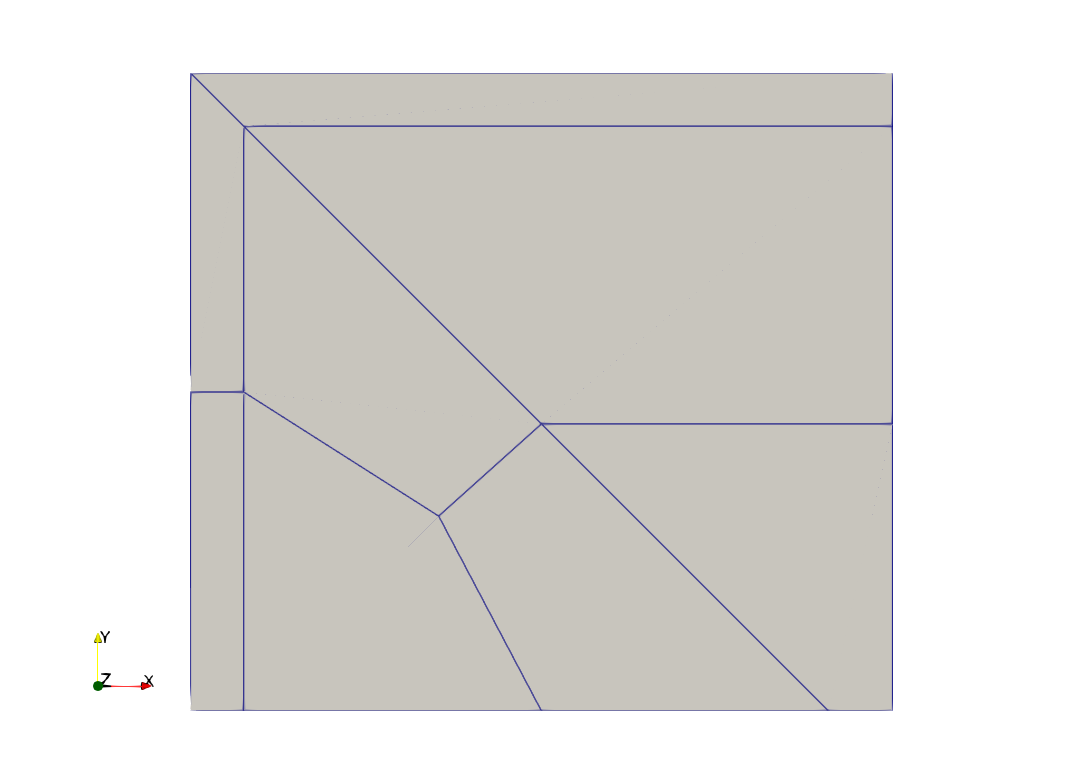
\includegraphics[width=8cm]{python_codes/fieldstone_149/results/mesh}
\end{center}

We then proceed by creating 8 blocks of resolution $10\times 10$. 
We then map them and finally assemble them one by one to obtain:

\begin{center}
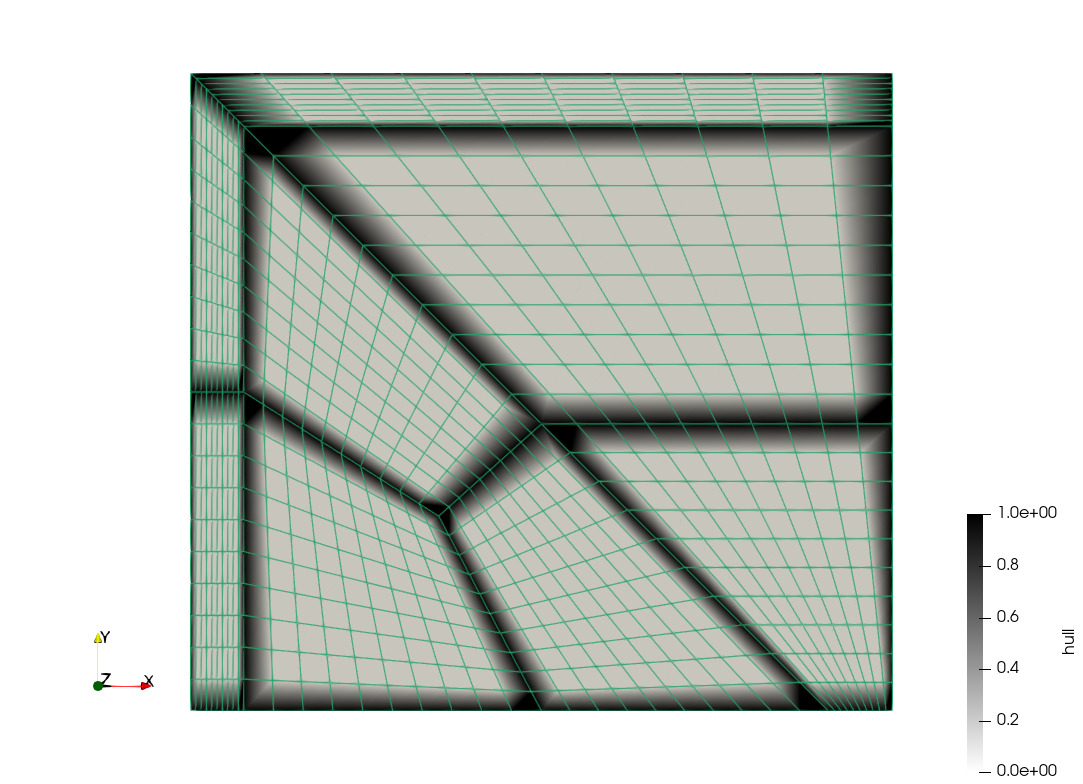
\includegraphics[width=8cm]{python_codes/fieldstone_149/results/vkkmesh}
\end{center}

The code uses analytical velocity from corner flow theory, 
and uses Q1 elements for temperature.

\begin{center}
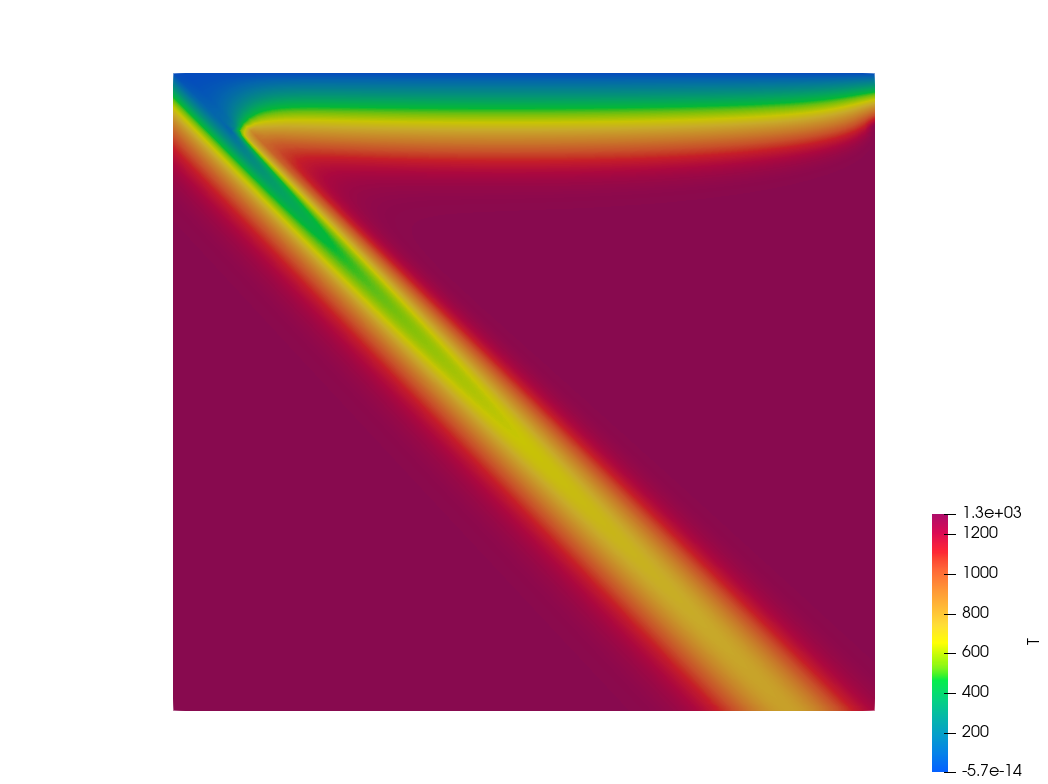
\includegraphics[width=8cm]{python_codes/fieldstone_149/results/temp}
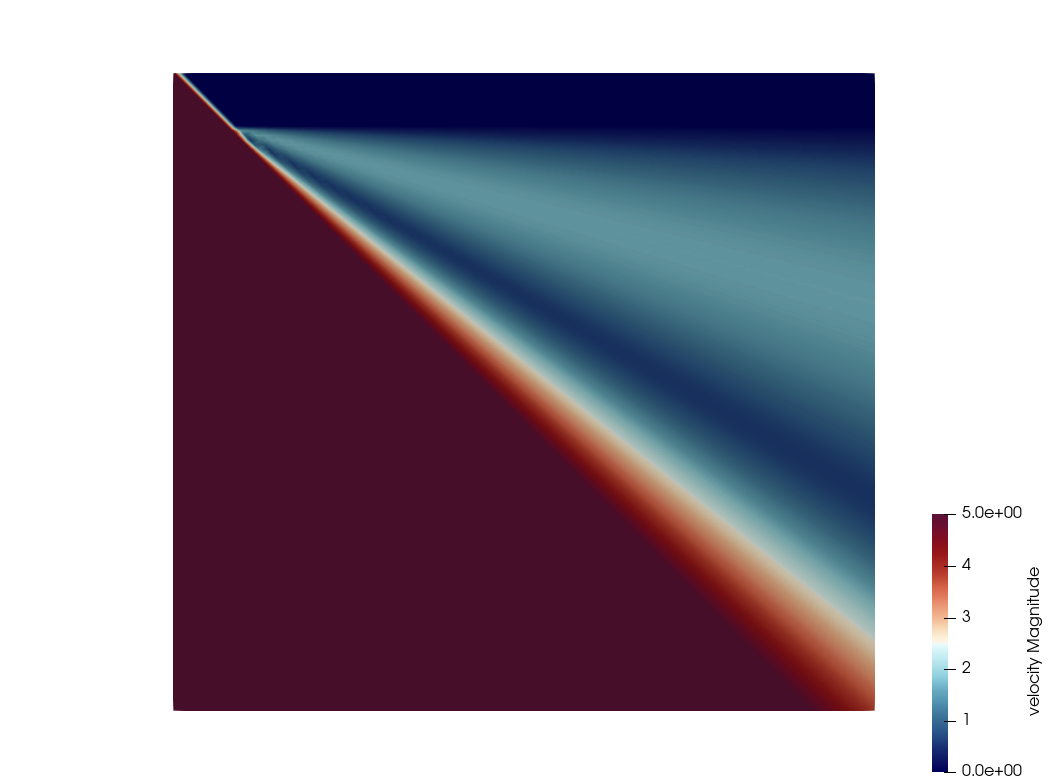
\includegraphics[width=8cm]{python_codes/fieldstone_149/results/vel}
\end{center}





%%%%%%%%%%%%%%%%%%%%%%%%%%%%%%%%%%%%%%%%%%%%%%%%%%%%%%%%%%%%%%%%%%%%%%%%%%%%%%%%%%%%%%%%%%%%%%%%%%%
\par\noindent\rule{\textwidth}{0.4pt}

\vspace{.5cm}

\begin{center}
\fbox{\begin{minipage}{0.9\textwidth}
{\color{teal}To Do, open questions, future work?}
\begin{itemize}
\item use f131 P1 to P2 tool to make Q1 to Q2 ?
\item redo figures with appropriate colors
\item redo (some) benchmark measurements?
\end{itemize}
\end{minipage}}
\end{center}

%%%%%%%%%%%%%%%%%%%%%%%%%%%%%%%%%%%%%%%%%%%%%%%%%%%%%%%%%%%%%%%%%%%%%%%%%%%%%%%%%%%%%%%%%%%%%%%%%%%
\vspace{.5cm}

\Literature:\\
\fullcite{vack08}\\
\fullcite{vatc23}

